\begin{frame}{Introduction}

\begin{itemize}
    \item To defend the potential threat from large-scale quantum computers, the US National Institute of Standards and Technology (NIST) initiated standardization process for post-quantum cryptography in 2016.
    \pause
    \item In 2022, four selected algorithms – CRYSTALS-Kyber, CRYSTALS-Dilithium, \textsc{Falcon}, and SPHINCS+ were expected to be part of NIST's post-quantum cryptographic standards.
    \pause
    \item  In theory, these algorithms can base their security on problems that are considered still hard given the advantage of quantum computing.
    \pause
    \item In practice, the implementations of these algorithms can suffer side-channel attacks.
\end{itemize}

\end{frame}


\begin{frame}{Side-channel Attacks on \textsc{Falcon}}

%\begin{figure}
%    \centering
%    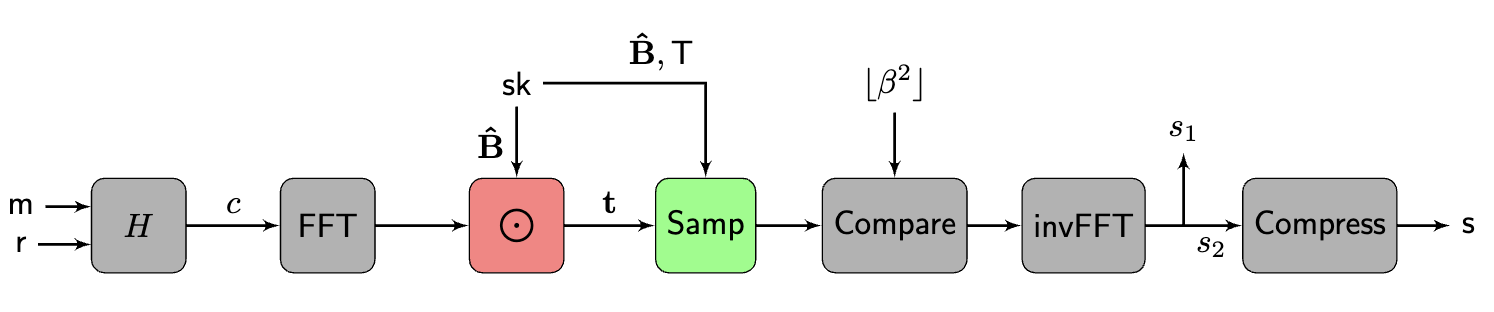
\includegraphics[width=\textwidth]{tikz/falcon-sign.png}
%    \caption{A graphical overview of {\sf FALCON.Sign}}
%    \label{fig:enter-label}
%\end{figure}

\begin{figure}
\centering

% \begin{tikzpicture}[node distance=2cm, gridded]
\begin{tikzpicture}[node distance=2cm]

% Gadgets
\node (hash) [rectangle, rounded corners, 
minimum width=1cm, 
minimum height=1cm,
text centered,
fill=white!70!black,
draw=black] at (0,0) {$H$};
\coordinate (hash-in1) at ($(hash) + (-0.5,0.2)$);
\coordinate (hash-in2) at ($(hash) + (-0.5,-0.2)$);


\node (FFT) [rectangle, rounded corners, 
minimum width=1cm, 
minimum height=1cm,
text centered,
fill=white!70!black,
draw=black, right of=hash, xshift=-0.5cm] {{\sf FFT}}; 

\node (point-mult) [rectangle, rounded corners, 
minimum width=1cm, 
minimum height=1cm,
text centered, 
fill=white!50!red,
draw=black, right of=FFT, xshift=-0.5cm] {$\bigodot$};
\coordinate (point-mult-in1) at ($(point-mult) + (-0.5,0.2)$);
\coordinate (point-mult-in2) at ($(point-mult) + (-0.5,-0.2)$);

\node (samp) [rectangle, rounded corners, 
minimum width=1cm, 
minimum height=1cm,
text centered, 
fill=white!50!green,
draw=black, right of=point-mult] {{\sf Samp}};
\coordinate (samp-in1) at ($(samp) + (-0.5,0.2)$);
\coordinate (samp-in2) at ($(samp) + (-0.5,-0.2)$);

\node (compare) [rectangle, rounded corners, 
minimum width=1cm, 
minimum height=1cm,
text centered, 
fill=white!70!black,
draw=black, right of=samp] {{\sf Compare}};

\node (invFFT) [rectangle, rounded corners, 
minimum width=1cm, 
minimum height=1cm,
text centered, 
fill=white!70!black,
draw=black, right of=compare] {${\sf invFFT}$};
\coordinate (invFFT-out1) at ($(invFFT.east) + (0,0.2)$);
\coordinate (invFFT-out2) at ($(invFFT.east) + (0,-0.2)$);

\node (compress) [rectangle, rounded corners, 
minimum width=1cm, 
minimum height=1cm,
text centered, 
fill=white!70!black,
draw=black, right of=invFFT] {{\sf Compress}};


% Texts
\node (m) at ($(hash-in1) + (-0.75,0)$) {{\sf m}};
\node (r) at ($(hash-in2) + (-0.75,0)$) {{\sf r}};
% \node (B) at ($(point-mult-in1) + (-1.5,0)$) {$\mathbf{\hat B}$};
\node (sk) at ($(point-mult.north) + (0,1)$) {$\sf sk$};
% \node (beta) at ($(compare.north) + (0,1)$) {$\lfloor \beta^2 \rfloor$};
% \node (s1) at ($(invFFT.east) + (0.4,1)$) {$s_1$};
\node (s) at ($(compress.east) + (0.75,0)$) {$\sf s$};

% Lines
\draw [arrow] (m) -- (hash-in1);
\draw [arrow] (r) -- (hash-in2);
\draw [arrow] (hash.east) -- node[above]{} (FFT.west);

\draw [arrow] (FFT.east) -- (point-mult.west);
\draw [arrow] (sk) -- node[left]{} (point-mult.north);

\draw [arrow] (point-mult.east) -- node[above]{} (samp.west);
\draw [arrow] (sk) -| node[above left]{} (samp.north);

\draw [arrow] (samp.east) -- (compare.west);

% \draw [arrow] (beta) -- (compare.north);

\draw [arrow] (compare.east) -- (invFFT.west);

\draw [arrow] (invFFT.east) -- (compress.west);
% \draw [arrow] (invFFT.east) -| node[below right]{$s_2$} (s1);

\draw [arrow] (compress.east) -- (s);


\end{tikzpicture}

\caption{A graphical overview of {\sf FALCON.Sign}.}
\label{fig:falcon-sign-test}
\end{figure}


\begin{center}
{\small
\begin{tabular}{ l | c | c }
 & Attack & Countermeasure \\
\hline
\makecell{{\color{red}Pre-image Vector Computation}} & \cite{KA21, TCHES:GMRR22} & \textcolor<2>{red}{None} \\
\hline
\makecell{{\textcolor{black!30!green}{Gaussian Sampler over Lattices}}} & \cite{TCHES:GMRR22, EC:ZLYW23} & \cite{TCHES:GMRR22, EC:ZLYW23} \\ 
\end{tabular}
}
\end{center}
    
\end{frame}


\begin{frame}{Our Contributions}

In this paper, we present the following contributions:
\pause
\begin{itemize}
    \item We propose the first masking scheme on the floating-point number multiplication and addition in the pre-image vector computation of \textsc{Falcon} as a countermeasure.
    \pause
    \item We verify higher-order security of our design in the probing model.
    \pause
    \item To test the practical leakage of our work, we conduct the Test Vector Leakage Assessment (TVLA) \cite{gilbert2011testing} experiments.
    \pause
    \item We also test the performance by comparing with the reference implementation of \textsc{Falcon} \cite{NISTPQC-R3:FALCON20}.
\end{itemize}


\end{frame}


\begin{frame}{Notation}

Throughout the presentation, we assume
\pause
\begin{itemize}
%    \item $M > N$ are two positive integers and $N = 2^\kappa$ for some integer $\kappa$.
%    \pause
%    \item $\phi = x^N + 1$ is a polynomial.
%    \pause
%    \item $q$ is a prime number.
%    \pause
%    \item Represent a vector $\mathbf{v}$ by a boldface letter, and a matrix $\mathbf{A}$ by a boldface capital letter.
%    \item For a polynomial $f \in \Z[x] / \phi$, it can be considered as an $N$-by-$N$ matrix.
    \item For a variable $x$, the $j$th bit of $x$ is written as $x^{(j)}$.
    \pause
    \item The $i$th bit to $j$th bit ($j \geq i$) of $x$ is represented by $x^{[j:i]}$.
    \pause
    \item A sequence of $n$ variables $(x_1, x_2, \cdots, x_n)$ (e.g. shares of variable $x$) is written as $(x_i)_{1 \leq i \leq n}$, or simply $(x_i)$.
    \pause
    \item For a proposition $P$, $\llbracket P \rrbracket = 1$ if and only if $P$ is true and $0$ if otherwise.
\end{itemize}
    
\end{frame}
